\documentclass[journal,12pt,twocolumn]{IEEEtran}
\usepackage{graphicx}
\graphicspath{{./figs/}}{}
\usepackage{amsmath,amssymb,amsfonts,amsthm}
\newcommand{\myvec}[1]{\ensuremath{\begin{pmatrix}#1\end{pmatrix}}}
\providecommand{\norm}[1]{\lVert#1\rVert}
\usepackage{listings}
\usepackage{watermark}
\usepackage{titlesec}
\usepackage{caption}
\let\vec\mathbf
\lstset{
frame=single, 
breaklines=true,
columns=fullflexible
}
\thiswatermark{\centering \put(0,-105.0){
\includegraphics[scale=0.15]{/sdcard/IITH/vectors/10.7.2.5/figs/logo.png}} }
\title{\mytitle}
\title{
Assignment - Vector-2
}
\author{Surajit Sarkar}
\begin{document}
\maketitle
\tableofcontents
\bigskip
\section{\textbf{Problem}}
Find the ratio in which the line segment joining A(1, – 5) and B(– 4, 5) is divided by the
x-axis. Also find the coordinates of the point of division.
\section{\textbf{Solution}}
Let the x-axis divide the line segment at point (x,0) in the ratio k:1.
\begin{align}
\vec{A}&=\myvec{1 \\ -5} \\ 
\Vec{B}&=\myvec{-4 \\ 5} \\ 
\Vec{X}&=\myvec{x\\0}
\end{align}
Using section formula,
\begin{align}
\vec{X}&=\frac{k\vec{B}+\vec{A}}{k+1}\\
\myvec{x\\0}&=\frac{k\myvec{-4\\5}+\myvec{1\\-5}}{k+1}\\
&=\myvec{-4k+1\\5k-5}\frac{1}{k+1}\\
&\Rightarrow \frac{5k-5}{k+1}=0\\
&\Rightarrow 5k=5\\
&\Rightarrow k=1
\end{align}
Find the coordinates of the point of division
\begin{align}
    \myvec{x\\0}&=\frac{\vec{B}+\vec{A}}{2}\\
    &=\myvec{-\frac{3}{2}\\0}
\end{align}
\section{\textbf{Code Link}}
\begin{lstlisting}
https://github.com/sssurajit/fwc/blob/main/vectors/10.7.2.5/codes/vector.py
\end{lstlisting}
Execute the code by using the command\\
\textbf{python3 vector.py}
\section{\textbf{Figure}}
\begin{figure}[!h]
\centering
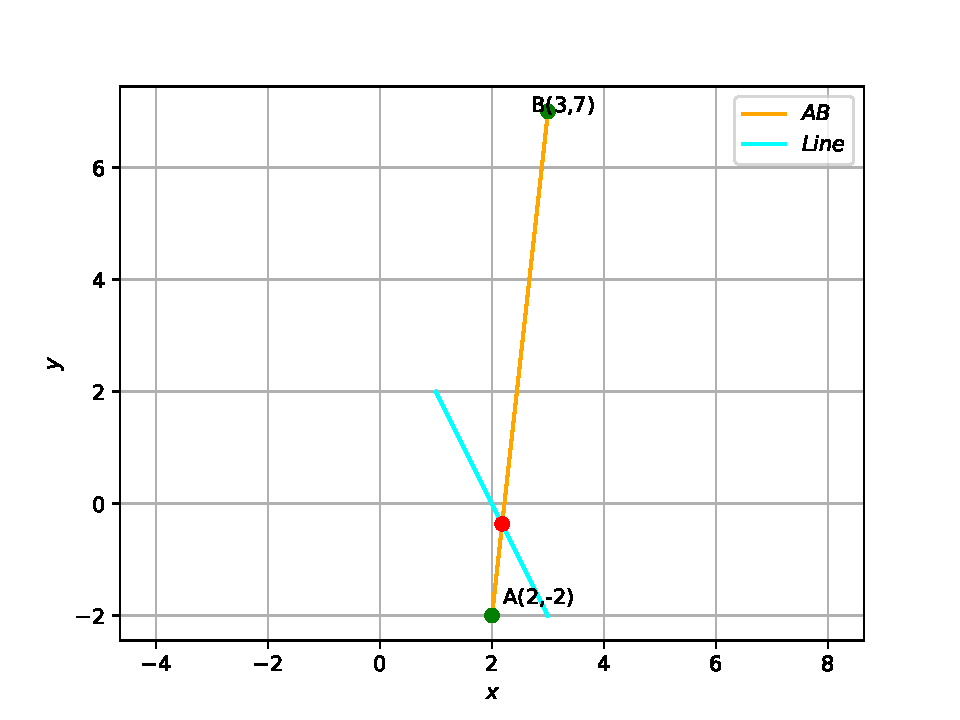
\includegraphics[width=\columnwidth]{/sdcard/IITH/vectors/10.7.2.5/figs/vec.pdf}
\caption{}
\label{fig:vec}
\end{figure}
\end{document}

